\documentclass[pdf]{prosper}
\usepackage[utf8x]{inputenc}
\usepackage[italian]{babel}
\usepackage[capsules]{HA-prosper}
\usepackage{lscape}
\usepackage{natbib}
\title{Linguistica dei corpora: una breve introduzione}
\author{Luigi Talamo (luigi.talamo@unibg.it)\\ \institution{Dottorato in Scienze Linguistiche: Università degli Studi di Bergamo e Università degli Studi di Pavia}}

\newcommand{\dxarr}{\begin{math}\rightarrow  \end{math}\hspace{1pt}}
\newcommand{\sxarr}{\begin{math}\leftarrow  \end{math}\hspace{1pt}}
\begin{document}
\maketitle

\begin{tsectionandpart}{CL: cos'è, teoria vs. metodologia, type/token, collocazione, frequenza e produttività}

\begin{slide}{Cos'è}

La linguistica dei corpora ({\it Corpus Linguistics}: CL) è lo studio del linguaggio così come lo si trova espresso in `campioni di lingua' (corpora).

Seguendo qualche suggestione naturalistica, lo possiamo paragonare all'esame dei campioni che viene effettuato nelle scienze naturali e della vita, come i campioni di sangue per la medicina e i carotaggi in geologia.

\end{slide}

\begin{slide}{Teoria o metodologia?}
	E' la domanda con cui si apre \citealt{Gries2009}, sul quale questo seminario è largamente basato.

Tra i linguisti dei corpora, gli approcci le risposte sono differenti:

\begin{itemize}
\item taluni, come Geoffrey Leech, considerano la CL una vera e propria `filosofia del linguaggio';
\item altri, probabilmente la maggioranza, trattano la CL come un `semplice' strumento di indagine e di analisi.
\end{itemize}

\end{slide}

\begin{slide}{CL come teoria}
Se consideriamo la CL come teoria, dovremmo poter elaborare una spiegazione al linguaggio (e di conseguenza una grammatica) basandoci solo sui dati del campione linguistico.

E' l'oggetto della {\it corpus-driven linguistics}: 

\begin{itemize}
\item uno dei principali obiettivi del trattamento automatico del linguaggio è quello di insegnare alle macchine il linguaggio naturale somministrando loro grosse quantità di dati linguistici;
\item discipline più teoriche come la semantica distribuzionale cercano di catturare i significati delle parole dai contesti in cui si trovano: ``You shall know a word by the company it keeps'' (Joseph Rupert Firth)
\end{itemize}

\end{slide}

\begin{slide}{CL come metodologia di indagine}
Considerare la CL come `semplice' metodologia di indagine non vuol dire affatto ridurre la sua portata a `mero strumento'; tuttavia, se la CL non è teoria di per sé, a quale sistema teorico la possiamo riferire?

\begin{itemize}
	\item alcune discipline linguistiche semplicemente non si {\it curano} di avere o di esplicitare basi teoriche: la maggior parte dei dizionari contemporanei è basata su corpora linguistici, così come molte opere di linguistica applicata e didattica delle lingue;
	\item la CL è ormai lo strumento di base della linguistica cognitiva e di stampo funzionalista, cioè di una linguistica basata sull'uso effettivo che i parlanti fanno della lingua ({\it usage-based cognitive-linguistic theories}). In questo senso, la CL si oppone anche teoricamente alla linguistica di stampo generativista, che è tradizionalmente basata sull'analisi del proprio ( = del linguista) linguaggio.
\end{itemize}
\end{slide}

\begin{slide}{CL e teorie costruttiviste}
L'uso della lingua da parte dei parlanti è uno dei pilastri fondamentali di una linguistica molto {\it à la page}, ovvero della linguistica di impianto costruttivista ({\it constructional grammar}. 

	Esistono almeno una mezza dozzina di teorie costruttiviste: la Construction Grammar (\citealt{Goldberg2013}), la Radical Construction Grammar (\citealt{Croft2001}), la Construction Morphology (\citealt{Booij2010}), \dots

Un altro pilastro fondamentale di queste teorie è ovviamente la costruzione, identificata come un unità fondamentale di forma e significato, che include in sé le tradizionali categorie linguistiche di morfema, parola, sintagma, ecc.

	\begin{itemize}
		\item Cagliari;
		\item cagliaritano;
		\item acchiappa-titolo;
		\item macchina da scrivere.
    	\end{itemize}

Da un punto di vista teorico la CL ha come unità fondamentale la collocazione.
\end{slide}

\begin{slide}{Type, token e collocazione}

Espressione = morfema, parola, composto, parola complessa, frase -> in CL `type'

Occorrenze = tutte le volte in cui trovo una data espressione su un corpus -> in CL `token'

Collocazione = insieme dei contesti di un corpus in cui si trova una data espressione, cioè insieme delle occorrenze

Esempio: 263 token del type `paludato' sul corpus La Repubblica

\begin{center}
\includegraphics[width=11cm]{paludato}
\end{center}

\end{slide}

\overlays{6}{
\begin{slide}{Collocazioni di {\it paludato}}
Cosa scopriamo dalle (poche) collocazioni di {\it paludato} viste sopra? Abbastanza!

\begin{itemstep}
\xitemwait
\xitem è un aggettivo: si accorda per genere e numero col nome a cui si riferisce ed è gradabile;
\xitem si può riferire sia ad un essere umano che ad un oggetto;
\xitem può reggere un argomento: {\it in sete arancioni...};
\xitem ha un (generico) significato di `solenne'... 
\xitem ...ma anche di `goffo, inadatto'.
\end{itemstep}

	La collocazione di una espressione ci svela le sue caratteristiche grammaticali (formali) e il suo significato, proprio come la costruzione è la rappresentazione della forma e del significato di una espressione.


\end{slide}
}

\overlays{5}{
\begin{slide}{Frequenza}
Nella sua accezione più semplice, la frequenza è la somma aritmetica delle collocazioni, cioè: l'espressione X si trova Y nel corpus Z.

\begin{itemstep}
\xitemwait
\xitem auto di piazza: ?
\xitem non la conosco: tre espressioni distinte. Auto che si prende in piazza? A noleggio?
\xitem 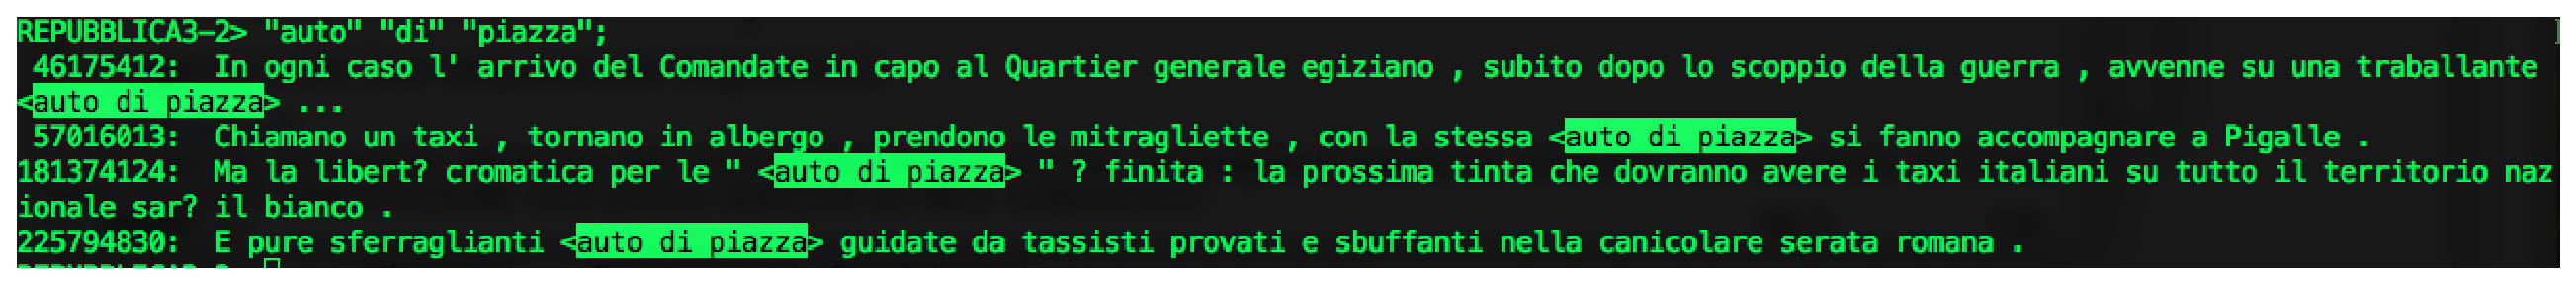
\includegraphics[width=11cm]{autodipiazza}
\xitem ora la conosco: una unica espressione (`parola')
\end{itemstep}
\end{slide}
}

\begin{slide}{Frequenza come {\it entrenchment}}
	Il concetto di frequenza è nuovamente un concetto che ha un corrispettivo funzionale nella linguistica cognitiva.
	
	Più alta è la frequenza, maggiore è la possibilità che una data costruzione sia immagazzinata (radicata) nel lessico mentale dei parlanti.

	\begin{itemize}
		\item se l'espressione è immagazzinata nel lessico, non la devo scomporre: <auto di piazza>;
		\item se non è immagazzinata, la devo analizzare `al volo': <auto> <di> <piazza>.

	\end{itemize}
\end{slide}

\end{tsectionandpart}

\begin{tsectionandpart}{CL al lavoro: qualche applicazione}

\overlays{5}{
\begin{slide}{Introduzione}
	Oltre al lessico, che è il primo, tradizionale dominio di utilizzo della CL (ad es., i progetti lessicografici avviati dal De Mauro dagli anni settanta già utilizzavano dei corpora), la CL trova impiego in moltissimi altri campi legati alle scienze linguistiche:

	\begin{itemstep}
	\xitemwait 
	\xitem abbiamo già menzionato sopra dizionari e usi didattici della CL;
	\xitem calcolare la produttività di una costruzione morfologica;
	\xitem predirre quali scelte sintattiche fanno i parlanti di una lingua (e perché): ad es., il congiuntivo italiano è veramente morto?
	\xitem identificare il reale utilizzo di due parole all'apparenza tra loro sinonimiche: es. di sopra, quando utilizziamo {\it auto di piazza} al posto di `taxi'? e {\it paludato} al posto di `solenne' o di `goffo'? 
	\end{itemstep}
	\end{slide}
}

\begin{slide}{Costruzioni morfologiche: frequenza e produttività}
Facciamo ora il caso delle costruzioni morfologiche di tipo derivazionale, come le prefissazioni e le suffissazioni. Ad es., quanto e come i parlanti di lingua italiana utilizzano

	\begin{itemize}
		\item il suffisso {\it -ame}? legname, pietrame, bambiname, berlusconame, grillame 
		\item il prefissoide {\it tele-}? televendita, telecomando, telepresentatore
		\item il suffisoide {\it -poli}? tangentopoli, vallettopoli, guerciopoli
		\item il primo membro del composto {\it acchiappa-}? acchiappa-macchie, acchiappa-titoli
	\end{itemize}


ovvero: quanto e come è produttiva una data costruzione?

\end{slide}

\begin{slide}{Costruzioni morfologiche: type/token}
	Definire la frequenza e la produttività di una costruzione morfologica è un compito leggermente diverso dal definire gli stessi valori per una parola come {\it paludato} o {\it auto di piazza}.

Abbiamo detto prima che in CL una parola equivale ad un type, di cui troviamo un certo numero di token in un corpus.

Nelle costruzioni morfologiche ci troviamo di fronte a una regola - la costruzione, appunto - che crea:

	\begin{itemize}
	\item un certo numero di type diversi;
	\item ciascuno di questi type mostra un certo numero di token.
	\end{itemize}
\end{slide}

\begin{slide}{Tre tipi di produttività morfologica}
Per quanto riguarda le costruzioni morfologiche, \citealt{Baayen2009} distingue tre tipi di produttività:

	\begin{enumerate}
		\item produttività realizzata;
		\item produttività in espansione;
		\item produttività potenziale.
	\end{enumerate}	

\end{slide}

\begin{slide}{Produttività realizzata}
La produttività realizzata è il tipo più semplice di produttività e coincide di fatto con la frequenza dei types di una determinata costruzione morfologica.

Volendo fare un'analogia con l'economia, il primo tipo di produttività è simile alla fetta che ha una compagnia detiene sul mercato.

Se la produttività realizzata è alta, la costruzione morfologica avrà una grossa quota consolidata nel `mercato' delle derivazioni morfologiche.


	\begin{itemize}
		\item Come si calcola: Numero di types (costruzione)
	\end{itemize}

\end{slide}

\begin{slide}{Produttività in espansione}
Nel nostro paragone con l'economia di mercato, il secondo tipo di produttività misura quanto la costruzione morfologica si sta espandendo, anche a danno di altre derivazioni morfologiche. 

E' inoltre interessante notare che una costruzione può avere una scarsa produttività realizzata, ma un'alta produttività in espansione -> è il caso dei nuovi affissi

	\begin{itemize}
		\item Come si calcola. P = numero di hapax legomena (costruzione) / numero di hapax legomena (corpus)
	\end{itemize}

\end{slide}

\begin{slide}{Produttività potenziale}
Il terzo tipo di produttività misura quanto una costruzione morfologica è in grado di occupare una fetta di mercato; una azienda può essere anche in espansione, ma se il mercato è ormai saturo rischia probabilmente di fare bancarotta!

E' il tipo di produttività più utilizzato negli studi di CL e morfologia quantitativa, ed è chiamato semplicemente P:

\begin{itemize}
\item Come si calcola. P = numero di hapax legomena (costruzione) / numero di token totali (costruzione)
\end{itemize}

Con un aggiustamento a livello di sotto-corpora, l'indice P è utilizzato nei lavori di Gaeta \& Ricca sulla produttività dei suffissi italiani (\citealt{GaetaRicca2003}, \citealt{GaetaRicca2006}).
\end{slide}

\begin{slide}{Costruzioni morfologiche: esercizio}
Data la (reale) lista di frequenza della costruzione con {\it -ame} nel corpus La Repubblica, calcolare i tre tipi di produttività.

\end{slide}

\begin{slide}{Costruzioni sintattiche: type/token}
Per quanto riguarda la sintassi, abbiamo una certa costruzione che può essere espressa in diversi modi formali (type), ciascuno dei quali ha un certo numero di token.

Secondo il principio di non sinonimità, una differenza formale tra due costruzioni implica SEMPRE una differenza di significato: ``If two constructions are syntactically distinct, they must be semantically or pragmatically distinct'' (Adele Goldberg)

Ad es., l'inglese possiede due modi di esprimere la costruzione sintattica ditransitiva, cioè AZIONE QUALCOSA A QUALCUNO, dove AZIONE è un verbo come dare, portare, ecc. :

	\begin{itemize}
	\item Mary gives a letter to John;
	\item Mary gives John a letter.
	\end{itemize}

\end{slide}


\end{tsectionandpart}

\bibliography{ref}
\bibliographystyle{natbib}
\end{document}
